\documentclass[border=10pt]{standalone}

\usepackage{tikz}
\usepackage{tikzsymbols}
\usetikzlibrary{calc,patterns,shapes.geometric}

\def\centerarc[#1](#2)(#3:#4:#5){\draw[#1] ($(#2)+({#5*cos(#3)},{#5*sin(#3)})$) arc (#3:#4:#5);}

\begin{document}
	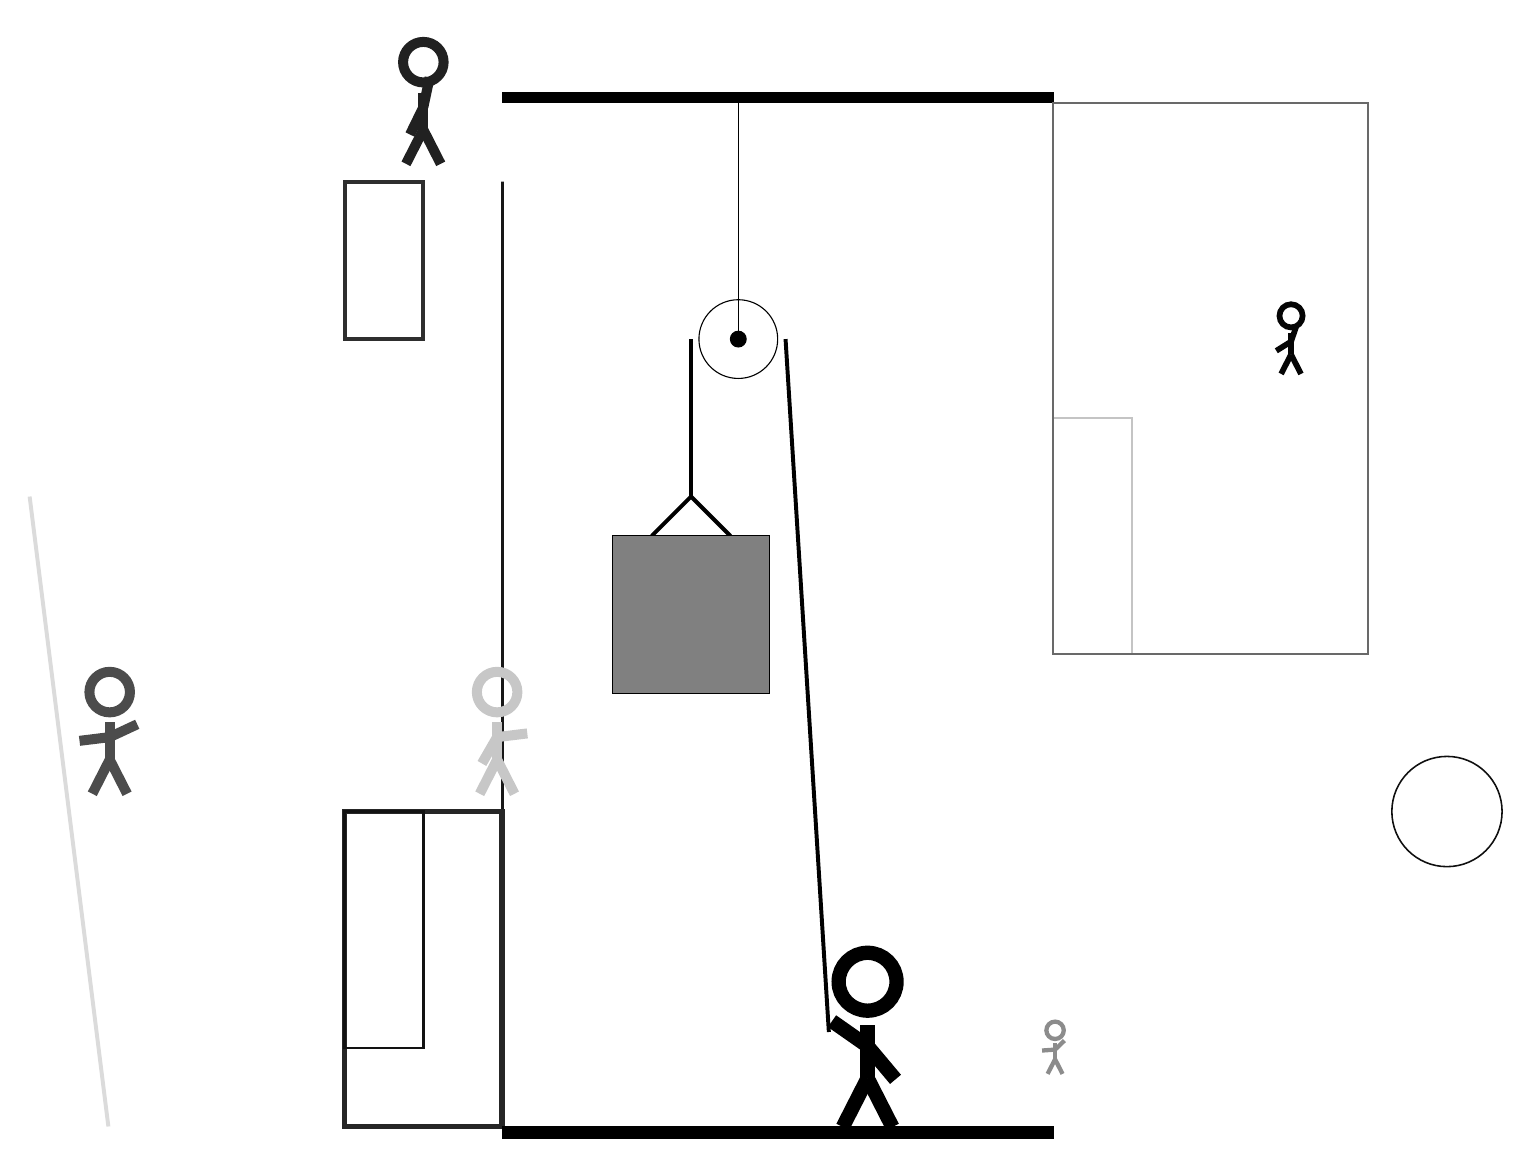
\begin{tikzpicture}
		%%%%% START %%%%%
		
		\draw[fill=black] (-2, 10) rectangle (5, 10.125);
		
		\draw (1, 7) circle (0.5);
		\draw[fill=black] (1, 7) circle (0.1);
		\draw (1, 10) -- (1, 7);
		
		\draw[line width=0.5mm] (-0.1, 4.5) -- (0.4, 5.0) -- (0.9, 4.5);
		\draw[fill=black!50] (-0.6, 4.5) rectangle (1.4, 2.5);
		
		\draw[line width=0.5mm] (0.4, 7) -- (0.4, 5.0);
		\centerarc[line width=0.5mm](1, 7)(0:180:0.6);
		\draw[line width=0.5mm](1.6, 7) -- (2.15, -1.8);
		
		\draw[line width=0.3mm, color=black!23] (5, 6) rectangle (6, 3);
		
		\draw[line width=0.2mm, color=black!59] (5, 10) rectangle (9, 3);
		\node[line width=0.6mm, color=black!87] at (-3, 10) {\Strichmaxerl[7][64][78]};
		\draw[line width=0.5mm, color=black!82] (-4, 9) rectangle (-3, 7);
		\draw[line width=0.4mm, color=black!91] (-2, 1) rectangle (-2, 9);
		\draw[line width=0.7mm, color=black!85] (-2, -3) rectangle (-4, 1);
		\node[line width=0.2mm, color=black!70] at (-7, 2) {\Strichmaxerl[7][7][25]};
		\node[line width=0.7mm, color=black!22] at (-2, 2) {\Strichmaxerl[7][60][7]};
		\node[line width=0.5mm, color=black!98] at (8, 7) {\Strichmaxerl[4][32][71]};
		\node[line width=0.4mm, color=black!45] at (5, -2) {\Strichmaxerl[3][4][44]};
		\draw [line width=0.2mm, color=black!94](10, 1) circle (0.7);
		\draw[line width=0.3mm, color=black!93] (-4, -2) rectangle (-3, 1);
		\draw[line width=0.5mm, color=black!14](-7, -3) -- (-8, 5);
		
		
		\node at (2.6, -1.9) {\Strichmaxerl[10][-35][-50]};
		
		\draw[fill=black] (-2, -3) rectangle (5, -3.15);
		
		%%%%% END %%%%%
	\end{tikzpicture}
\end{document}